\documentclass[tikz,border=15pt]{standalone}
\usepackage{tikz}
\usepackage{xcolor}
\usetikzlibrary{arrows.meta,calc}

\definecolor{wallgray}{RGB}{241,245,249}
\definecolor{woodfloor}{RGB}{253,230,138}
\definecolor{wooddark}{RGB}{180,83,9}
\definecolor{baseboard}{RGB}{203,213,225}
\definecolor{windowblue}{RGB}{186,230,253}
\definecolor{posterbg}{RGB}{15,23,42}
\definecolor{postergold}{RGB}{250,204,21}
\definecolor{posterrose}{RGB}{244,63,94}
\definecolor{hoodieorange}{RGB}{249,115,22}
\definecolor{jeansblue}{RGB}{30,58,138}
\definecolor{skincolor}{RGB}{254,215,170}
\definecolor{vrblue}{RGB}{56,189,248}
\definecolor{vrcyancyber}{RGB}{0,242,254}
\definecolor{motherdress}{RGB}{168,85,247}
\definecolor{apronyellow}{RGB}{254,240,138}
\definecolor{slipperspink}{RGB}{236,72,153}
\definecolor{motherhair}{RGB}{88,47,14}
\definecolor{doorframe}{RGB}{120,53,15}
\definecolor{sightgold}{RGB}{245,158,11}
\definecolor{deskwood}{RGB}{148,163,184}
\definecolor{pcslate}{RGB}{30,41,59}
\definecolor{pcscreen}{RGB}{30,27,75}
\definecolor{pcdark}{RGB}{15,23,42}
\definecolor{bedblue}{RGB}{59,130,246}
\definecolor{bedsheet}{RGB}{96,165,250}
\definecolor{smilered}{RGB}{234,88,12}

\begin{document}
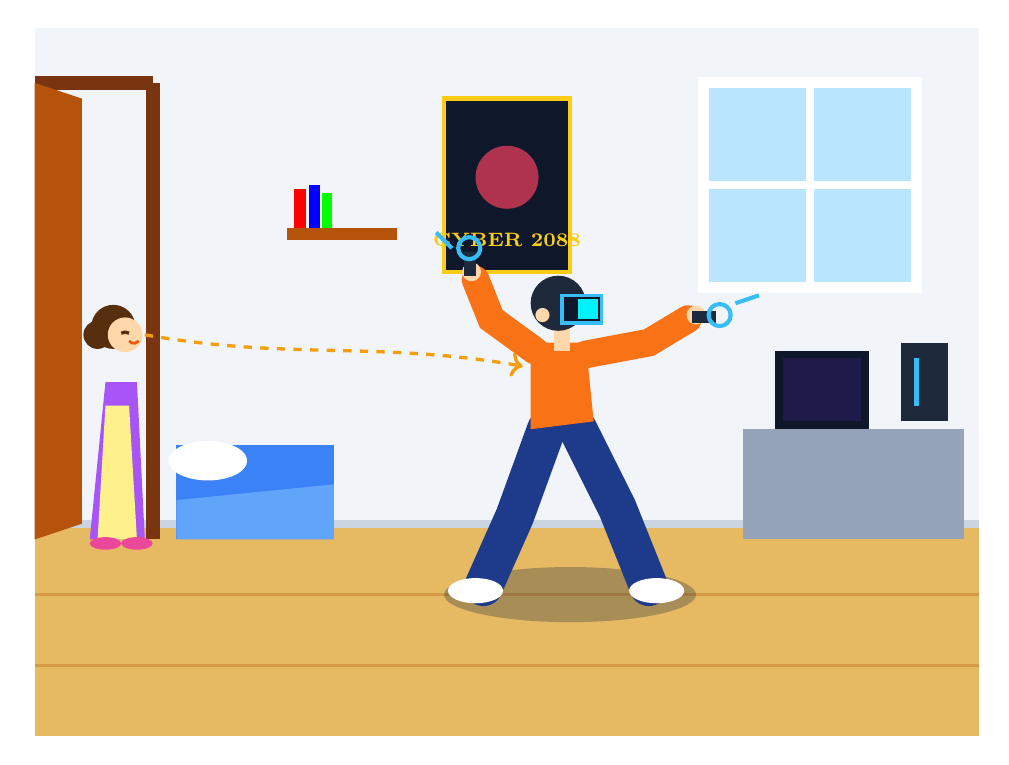
\begin{tikzpicture}

% 1. ROOM WALL & FLOOR
\fill[wallgray] (-6,-4.5) rectangle (6,4.5);
\fill[woodfloor] (-6,-4.5) rectangle (6,-1.8);
\fill[wooddark, opacity=0.3] (-6,-4.5) rectangle (6,-1.8);
\fill[baseboard] (-6,-1.85) rectangle (6,-1.75);

% Floor lines
\draw[wooddark, opacity=0.3, line width=0.8pt] (-6,-2.7) -- (6,-2.7);
\draw[wooddark, opacity=0.3, line width=0.8pt] (-6,-3.6) -- (6,-3.6);

% 2. BEDROOM DECORATIONS
% Window (Top Right)
\fill[windowblue] (2.5, 1.2) rectangle (5.2, 3.8);
\draw[white, line width=4pt] (2.5, 1.2) rectangle (5.2, 3.8);
\draw[white, line width=3pt] (3.85, 1.2) -- (3.85, 3.8);
\draw[white, line width=3pt] (2.5, 2.5) -- (5.2, 2.5);

% Desk & PC (Right)
\fill[deskwood] (3.0, -2.0) rectangle (5.8, -0.6);
\fill[pcdark] (3.4, -0.6) rectangle (4.6, 0.4);
\fill[pcscreen] (3.5, -0.5) rectangle (4.5, 0.3);
\fill[pcslate] (5.0, -0.5) rectangle (5.6, 0.5);
\draw[vrblue, line width=1.5pt] (5.2, -0.3) -- (5.2, 0.3);

% Poster on Wall
\fill[posterbg] (-0.8, 1.4) rectangle (0.8, 3.6);
\draw[postergold, line width=1.5pt] (-0.8, 1.4) rectangle (0.8, 3.6);
\fill[posterrose, opacity=0.7] (0, 2.6) circle (0.4cm);
\node[text=postergold, font=\scriptsize\bfseries] at (0, 1.8) {CYBER 2088};

% Bookshelf (Left wall)
\fill[wooddark] (-2.8, 1.8) rectangle (-1.4, 1.95);
\fill[red] (-2.7, 1.95) rectangle (-2.55, 2.45);
\fill[blue] (-2.52, 1.95) rectangle (-2.38, 2.5);
\fill[green] (-2.35, 1.95) rectangle (-2.22, 2.4);

% Bed (Far Left)
\fill[bedblue] (-4.2, -2.0) rectangle (-2.2, -0.8);
\fill[white] (-3.8, -1.0) ellipse (0.5cm and 0.25cm);
\fill[bedsheet] (-4.2, -2.0) -- (-2.2, -2.0) -- (-2.2, -1.3) -- (-4.2, -1.5) -- cycle;

% 3. DOORWAY & MOTHER (Left)
\draw[doorframe, line width=5pt] (-4.5, -2.0) -- (-4.5, 3.8);
\draw[doorframe, line width=5pt] (-6.0, 3.8) -- (-4.5, 3.8);
\fill[wooddark] (-6.0, -2.0) -- (-5.4, -1.8) -- (-5.4, 3.6) -- (-6.0, 3.8) -- cycle;

% Mother standing in doorway
% Dress & Apron
\fill[motherdress] (-5.3, -2.0) -- (-4.6, -2.0) -- (-4.7, 0.0) -- (-5.1, 0.0) -- cycle;
\fill[apronyellow] (-5.2, -2.0) -- (-4.7, -2.0) -- (-4.8, -0.3) -- (-5.1, -0.3) -- cycle;
% Slippers
\fill[slipperspink] (-5.1, -2.05) ellipse (0.2cm and 0.08cm);
\fill[slipperspink] (-4.7, -2.05) ellipse (0.2cm and 0.08cm);
% Head & Hair
\fill[motherhair] (-5.0, 0.7) circle (0.28cm);
\fill[motherhair] (-5.2, 0.6) circle (0.18cm);
\fill[skincolor] (-4.85, 0.6) circle (0.22cm);
\draw[motherhair, line width=1.2pt] (-4.8, 0.62) arc (60:120:0.1);
\draw[smilered, line width=1pt] (-4.8, 0.52) arc (-140:-40:0.08);

% Sightline from mother to son
\draw[sightgold, dashed, line width=1.2pt, ->] (-4.6, 0.6) to[out=-10, in=170] (0.2, 0.2);

% 4. SON IN VR (Center)
% Ground shadow
\fill[pcslate, opacity=0.3] (0.8, -2.7) ellipse (1.6cm and 0.35cm);

% Dynamic Action Legs
\draw[jeansblue, line width=14pt, line cap=round, line join=round] (0.5, -0.6) -- (0.1, -1.7) -- (-0.3, -2.6);
\fill[white] (-0.4, -2.65) ellipse (0.35cm and 0.16cm);
\draw[jeansblue, line width=14pt, line cap=round, line join=round] (0.9, -0.6) -- (1.4, -1.6) -- (1.8, -2.6);
\fill[white] (1.9, -2.65) ellipse (0.35cm and 0.16cm);

% Torso (Orange Hoodie)
\fill[hoodieorange] (0.3, -0.6) -- (1.1, -0.5) -- (1.0, 0.5) -- (0.3, 0.5) -- cycle;

% Head & VR Visor
\fill[skincolor] (0.6, 0.4) rectangle (0.8, 0.7);
\fill[pcslate] (0.65, 1.0) circle (0.35cm);
\fill[skincolor] (0.45, 0.85) circle (0.09cm);

% VR Goggles
\fill[pcdark] (0.7, 0.75) rectangle (1.2, 1.1);
\draw[vrblue, line width=1.2pt] (0.7, 0.75) rectangle (1.2, 1.1);
\fill[vrcyancyber] (0.9, 0.8) rectangle (1.15, 1.05);

% Left Arm & Controller
\draw[hoodieorange, line width=10pt, line cap=round] (0.35, 0.4) -- (-0.2, 0.8) -- (-0.4, 1.3);
\fill[skincolor] (-0.45, 1.4) circle (0.12cm);
\fill[pcslate] (-0.55, 1.35) rectangle (-0.4, 1.65);
\draw[vrblue, line width=1.5pt] (-0.48, 1.7) circle (0.14cm);

% Right Arm & Controller
\draw[hoodieorange, line width=10pt, line cap=round] (1.0, 0.35) -- (1.8, 0.5) -- (2.3, 0.8);
\fill[skincolor] (2.4, 0.85) circle (0.12cm);
\fill[pcslate] (2.35, 0.75) rectangle (2.65, 0.9);
\draw[vrblue, line width=1.5pt] (2.7, 0.85) circle (0.14cm);

% Cyber Spark Effects
\draw[vrblue, line width=1.5pt] (-0.7, 1.7) -- (-0.9, 1.9);
\draw[vrblue, line width=1.5pt] (2.9, 1.0) -- (3.2, 1.1);

\end{tikzpicture}
\end{document}
